\documentclass{beamer}
\usepackage[utf8]{inputenc}
\usepackage[russian]{babel}
\usepackage{graphicx}

\usenavigationsymbolstemplate{}

\begin{document}

    \title{НИР, СПбАУ, осень 2013    
     \\ Применение современных технологий видеоадаптеров к визуализации геоландшафта}
    \author{Тураев Тимур \\ Руководитель: Жидков Евгений, SimEx}
    \date{19 декабря 2013 г.}

    \frame{\titlepage}

    \begin{frame}\frametitle{План}
        \begin{itemize}
        	\item О проекте
            \item Задачи
            \item Проблемы
            \item Результаты
            \item Полученные знания
        \end{itemize}
    \end{frame}
    
    \begin{frame}\frametitle{О проекте}
        \begin{itemize}
            \item	С появлением новых технологий, задача генерации ландшафта переносится с CPU на GPU
            \item	CPU освобождается для других задач
            \item	Tesselation Shader
        \end{itemize}
    \end{frame}
    
    \begin{frame}\frametitle{Работа современного графического конвейера}
	    \begin{center}
        	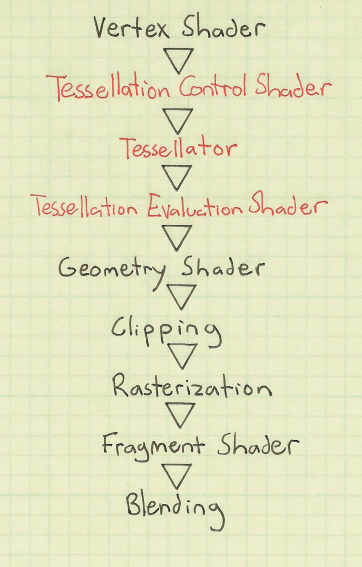
\includegraphics[scale=1.3]{ShaderStages.png}\\
        \end{center}
    \end{frame}

    \begin{frame}\frametitle{Задачи}
        \begin{itemize}%[<+->]
            \item   Изучить возможности конвейера OpenGL 4.0+
            \item   Применить тесселяционный шейдер для генерации ландшафта
            \item   (*) Визуализация поверхности Земли
        \end{itemize}
    \end{frame}
    
    \begin{frame}\frametitle{Проблемы}
        \begin{itemize}%[<+->]
            \item   Аппаратные проблемы (Intel GPU)
            \item   Программные проблемы (OS X, OpenGL version)
        \end{itemize}
    \end{frame}
    
    \begin{frame}\frametitle{Результаты}
        \begin{itemize}%[<+->]
            \item	В ускоренном режиме изучены основы OpenGL 4.0, языка GLSL; работа с библиотеками glew, glfw, glm, SOIL
            \item	Разобран новый конвеер растеризации, появившийся в OpenGL 4.0+
            \item	Написано небольшое тестовое приложение, демонстрирующая возможности GPU без использования CPU: изменение детализации поверхности в зависимости от расстояния от камеры.
        \end{itemize}
    \end{frame}

    \begin{frame}\frametitle{Поверхность}
        \begin{center}
        	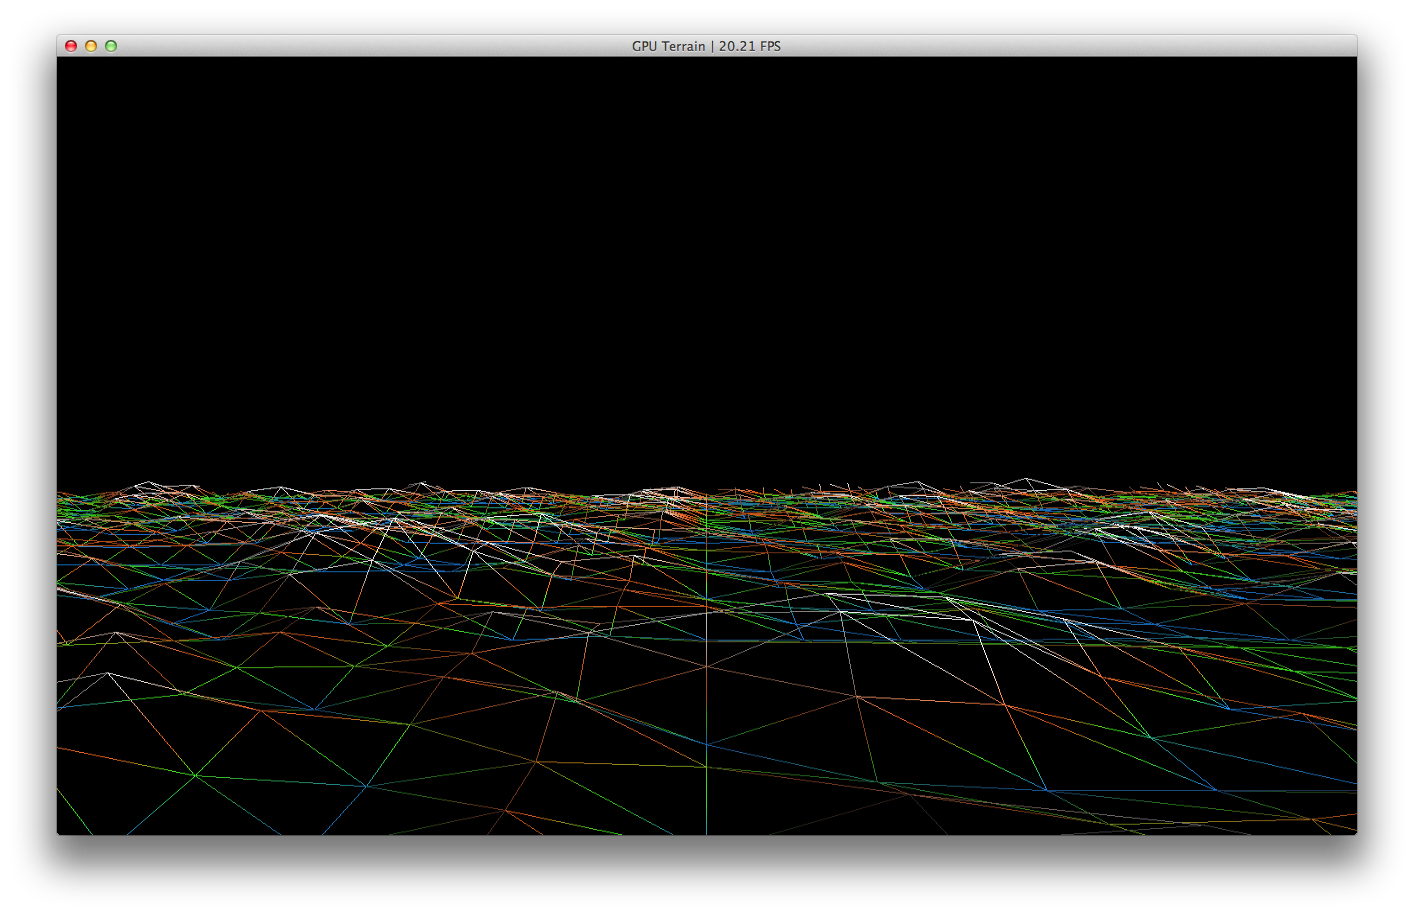
\includegraphics[scale=0.22]{1.png}\\
        \end{center}
    \end{frame}
    
    \begin{frame}\frametitle{Детализированная поверхность}
        \begin{center}
            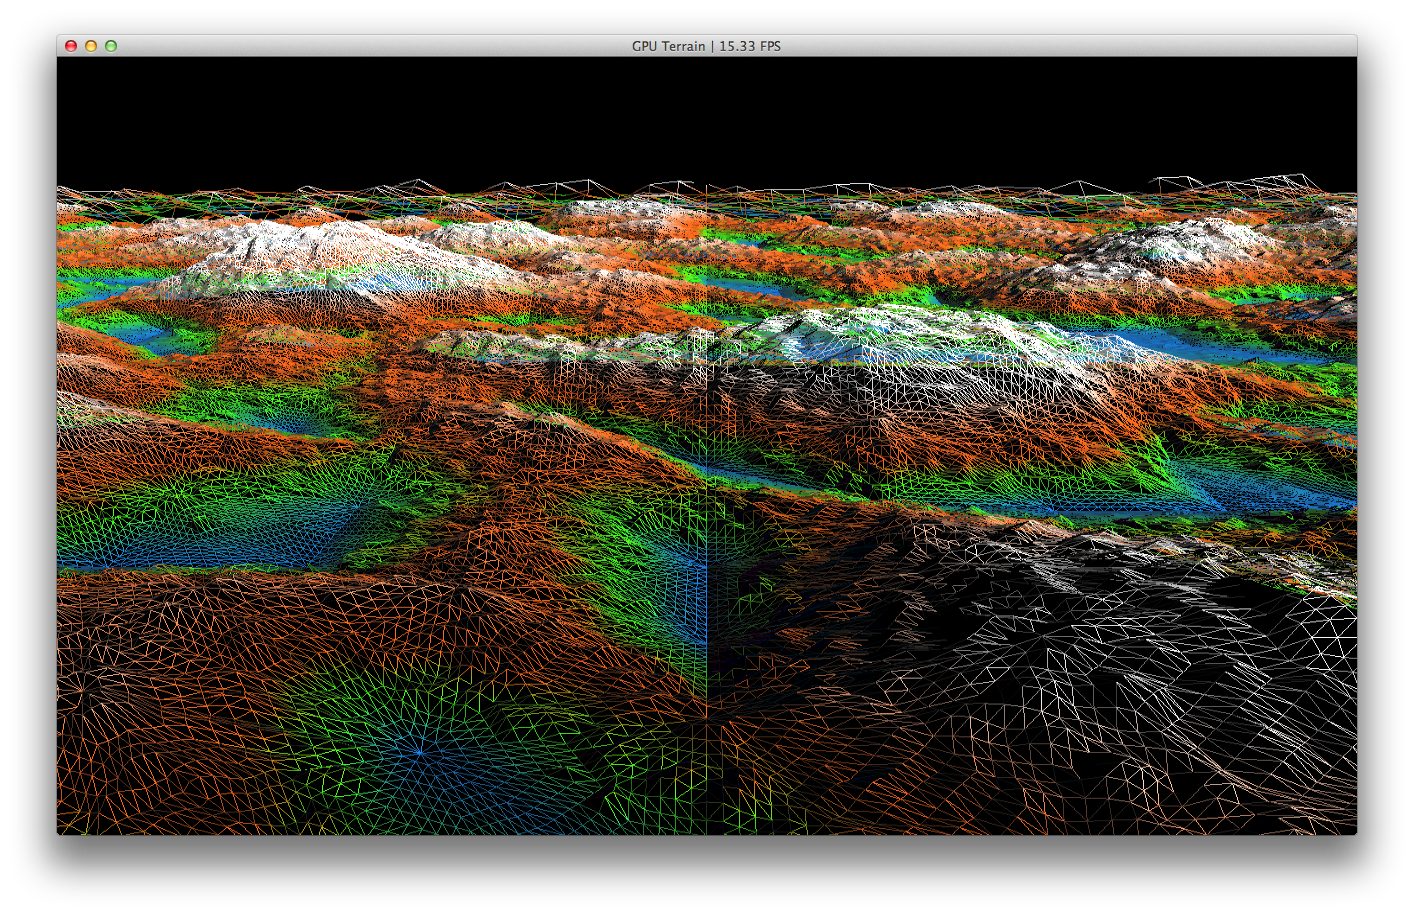
\includegraphics[scale=0.22]{2.png}\\
        \end{center}
    \end{frame}

    \begin{frame}\frametitle{Полученные знания}
        \begin{itemize}%[<+->]
            \item	Получены знания о технологии OpenGL, изучены возможности конвейера OpenGL 4.0+ (и его особенности в OS X)
            \item	Получены навыки работы с большим количеством библиотек и API.
        \end{itemize}
    \end{frame}

    \begin{frame}
        \begin{center}
            Спасибо за внимание!
        \end{center}
    \end{frame}

\end{document}
